\section{Theorie}
\label{sec:theorie}

In diesem Abschnitt sollen die theoretischen Grundlagen der Röntgenreflektometrie erläutert werden.
Dabei wird die Entstehung von Röntgenstrahlung erklärt,
sowie Besonderheiten bei der Reflexion der Strahlung an Oberflächen.

Röntgenstrahlung entsteht in einer Röntgenröhre,
welche aus einem Glaskolben besteht,
in dem sich eine Glühkathode,
sowie eine Anode befinden.
Mithilfe des glühelektrischen Effekts werden Elektronen erzeugt,
die in einem elektrischen Feld,
welches durch eine Beschleunigungsspannung zwischen Glühkathode und Anode vorliegt,
zur Anode hin beschleunigt werden.
Treffen die Elektronen auf die Anode,
werden sie stark abgebremst,
sodass Bremsstrahlung entsteht.
Des Weiteren übertragen sie ihre Energie an Elektronen in der Atomhülle der Anodenatome.
Die Hüllenelektronen können dabei aus dem Material herausgelöst werden,
sodass eine Lücke auf dem entsprechenden Niveau in der Atomhülle entsteht.
In diese Lücke kann ein höher gebundenes Elektron zurückfallen.
Die bei diesem Übergang freigesetzte,
diskrete Energie wird in Form eines Photons mit einer charakteristischen Wellenlänge freigesetzt.
Diese entstehenden Photonen bilden das charakteristische Spektrum der Röntgenstrahlung.
%Des Weiteren übertragen sie ihre Energie an Anodenatome,
%welche angeregt werden und schließlich Photonen mit einer charakteristischen Wellenlänge emittieren.
%Diese bilden das charakteristische Spektrum der Röntgenstrahlung.


\subsection{Reflexion von Röntgenstrahlung an Oberflächen}
\label{sec:reflexion_oberflaeche}

Beim Auftreffen einer elektromagnetischen Welle auf ein Medium mit einem anderen Brechungsindex wird ein Teil der Strahlung transmittiert,
während der andere Teil in einem Winkel von $\alpha_i = \alpha_f$ reflektiert wird.
Dies ist in \autoref{fig:mediumuebergang} gezeigt.
\begin{figure}
    \centering
    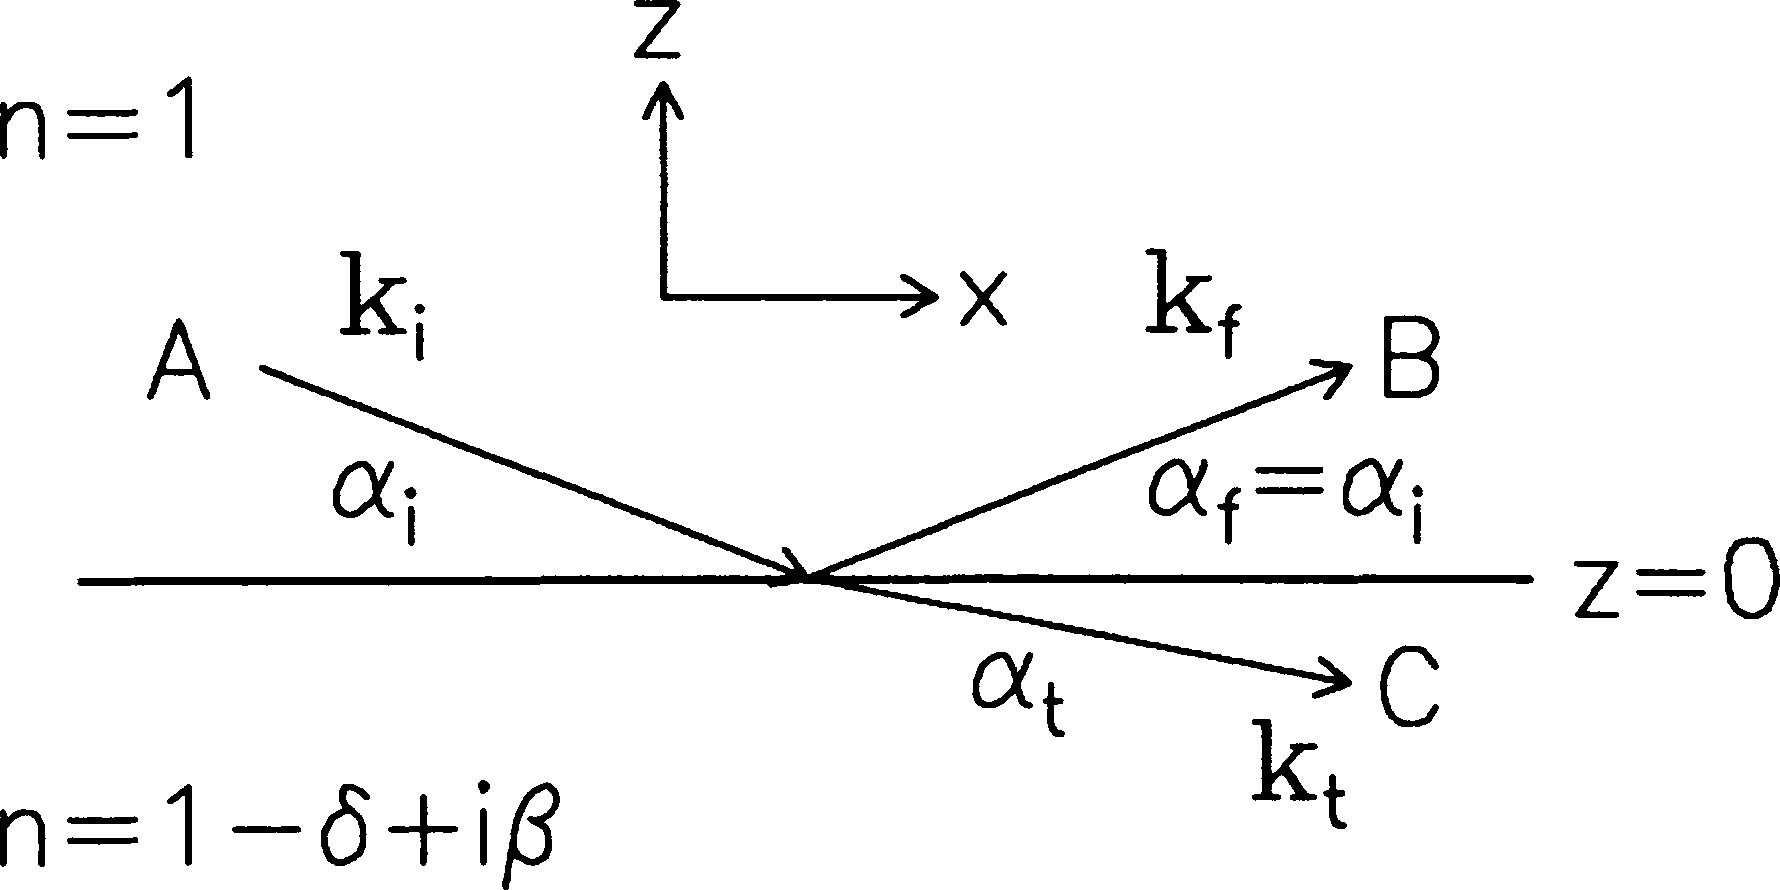
\includegraphics[width=0.6\textwidth]{content/img/Tolan_2.1.png}
    \caption{Transmission und Reflexion einer elektromagnetischen Welle an einer Grenzfläche zu einem Medium mit anderem Brechungsindex \cite{tolan}.}
    \label{fig:mediumuebergang}
\end{figure}
Der Anteil der reflektierten,
beziehungsweise transmittierten Amplitude zur einfallenden Amplitude wird mithilfe der Fresnel'schen Formeln beschrieben.
Im Fall von Röntgenstrahlung ist der Brechungsindex durch
\begin{equation}
    n = 1 - \delta + i \beta
    \label{eqn:brechungsindex}
\end{equation}
gegeben,
wobei $\delta$ die Dispersion und $\beta$ die Absorption beschreibt.
Da $\delta$ positiv ist und in einer Größenordnung von $\num{e{-6}}$ liegt,
ist der Brechungsindex für Röntgenstrahlung immer kleiner eins.
Aus diesem Grund können Unterschiede zwischen den Polarisationen der Strahlung vernachlässigt werden und aus den Fresnel'schen Formel folgen die Gleichungen
\begin{gather}
    t = \frac{2n_1}{n_1 \cos{\alpha_1} + n_2 \cos{\alpha_2}} \\
    r = \frac{n_1 \cos{\alpha_1} - n_2 \cos{\alpha_2}}{n_1 \cos{\alpha_1} + n_2 \cos{\alpha_2}}
\end{gather}
für den Transmissionskoeffizienten $t$ und den Reflexionskoeffizienten $r$.
Des Weiteren kann Totalreflexion auftreten,
was bedeutet,
dass der gesamte Anteil der einfallenden Strahlung reflektiert wird.
Diese ergibt sich unterhalb eines kritischen Winkels $\alpha_\text{c}$,
welcher sich näherungsweise durch
\begin{equation}
    \alpha_\text{c} \approx \sqrt{2 \delta} = \lambda \cdot \sqrt{\frac{r_\text{e} \rho}{\pi}}
\end{equation}
beschreiben lässt,
mit dem Elektronenradius $r_\text{e}$ und der Elektronendichte $\rho$.

Um zu gewährleisten,
dass der Strahl optimal auf die Oberfläche trifft und reflektiert wird,
muss ein Geometriefaktor $G$ berücksichtigt werden.
Es wird angenommen,
dass die Strahlung erst ab einem Einfallswinkel $\alpha_\text{g}$ vollständig auf die Probe trifft.
Bei kleineren Einfallswinkeln $\alpha_i < \alpha_\text{g}$ wird nur ein Teil der Strahlung reflektiert,
wie in \autoref{fig:geometriefaktor} dargestellt.
\begin{figure}
    \centering
    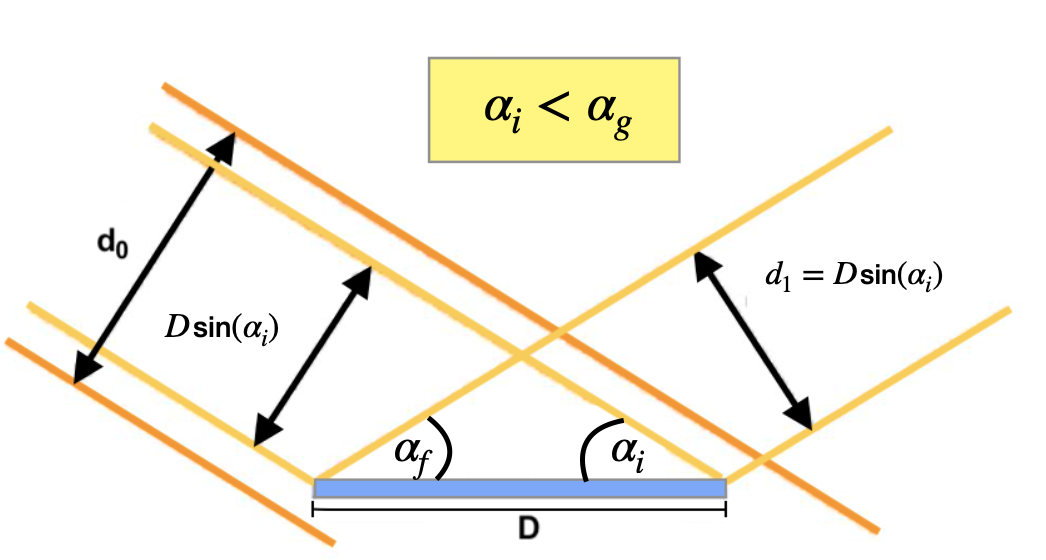
\includegraphics[width=0.5\textwidth]{content/img/Abb_7.png}
    \caption{Darstellung der Reflexion von Röntgenstrahlung mit einem Einfallswinkel $\alpha_i < \alpha_\text{g}$ \cite{versuchsanleitung}.
    Der Strahl trifft nicht vollständig auf die Probe und wird somit nicht vollständig reflektiert.}
    \label{fig:geometriefaktor}
\end{figure}
Für den Geometriefaktor gilt
\begin{equation}
    G =
    \begin{cases}
        \frac{D \sin{\alpha_i}}{d_0}, &\text{für} \ \alpha_i < \alpha_\text{g} \\
        1                           , &\text{für} \ \alpha_i > \alpha_\text{g} \ ,
    \end{cases}
    \label{eqn:geometriefaktor}
\end{equation}
wobei $D$ und $d_0$ die Durchmesser der Probe und des Röntgenstrahles beschreiben.


\subsection{Reflexion an Mehrschichtsystemen}

Bei Systemen von mehreren Schichten treten die in \autoref{sec:reflexion_oberflaeche} beschriebenen Phänomene der Reflexion und Transmission an jeder Schicht auf.
Dies ist in \autoref{fig:mehrschichtsystem} dargestellt.
\begin{figure}
    \centering
    \begin{subfigure}{0.48\textwidth}
        \centering
        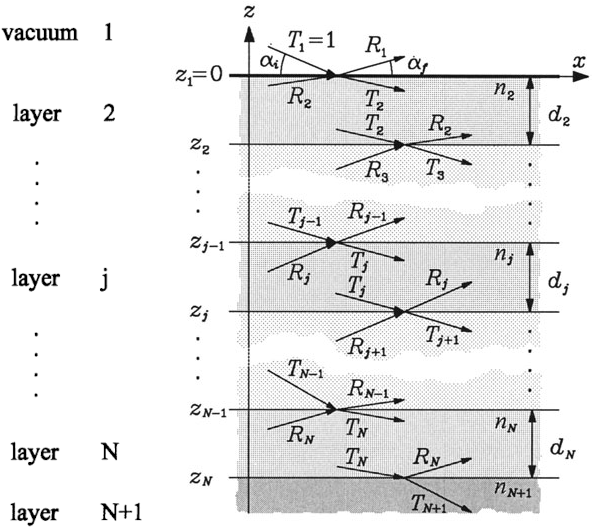
\includegraphics[width=\textwidth]{content/img/Tolan_2.6.png}
        \caption{Reflexion und Transmission in einem Mehrschichtsystem \cite{tolan}.}
        \label{fig:mehrschichtsystem}
    \end{subfigure}
    \hfill
    \begin{subfigure}{0.48\textwidth}
        \centering
        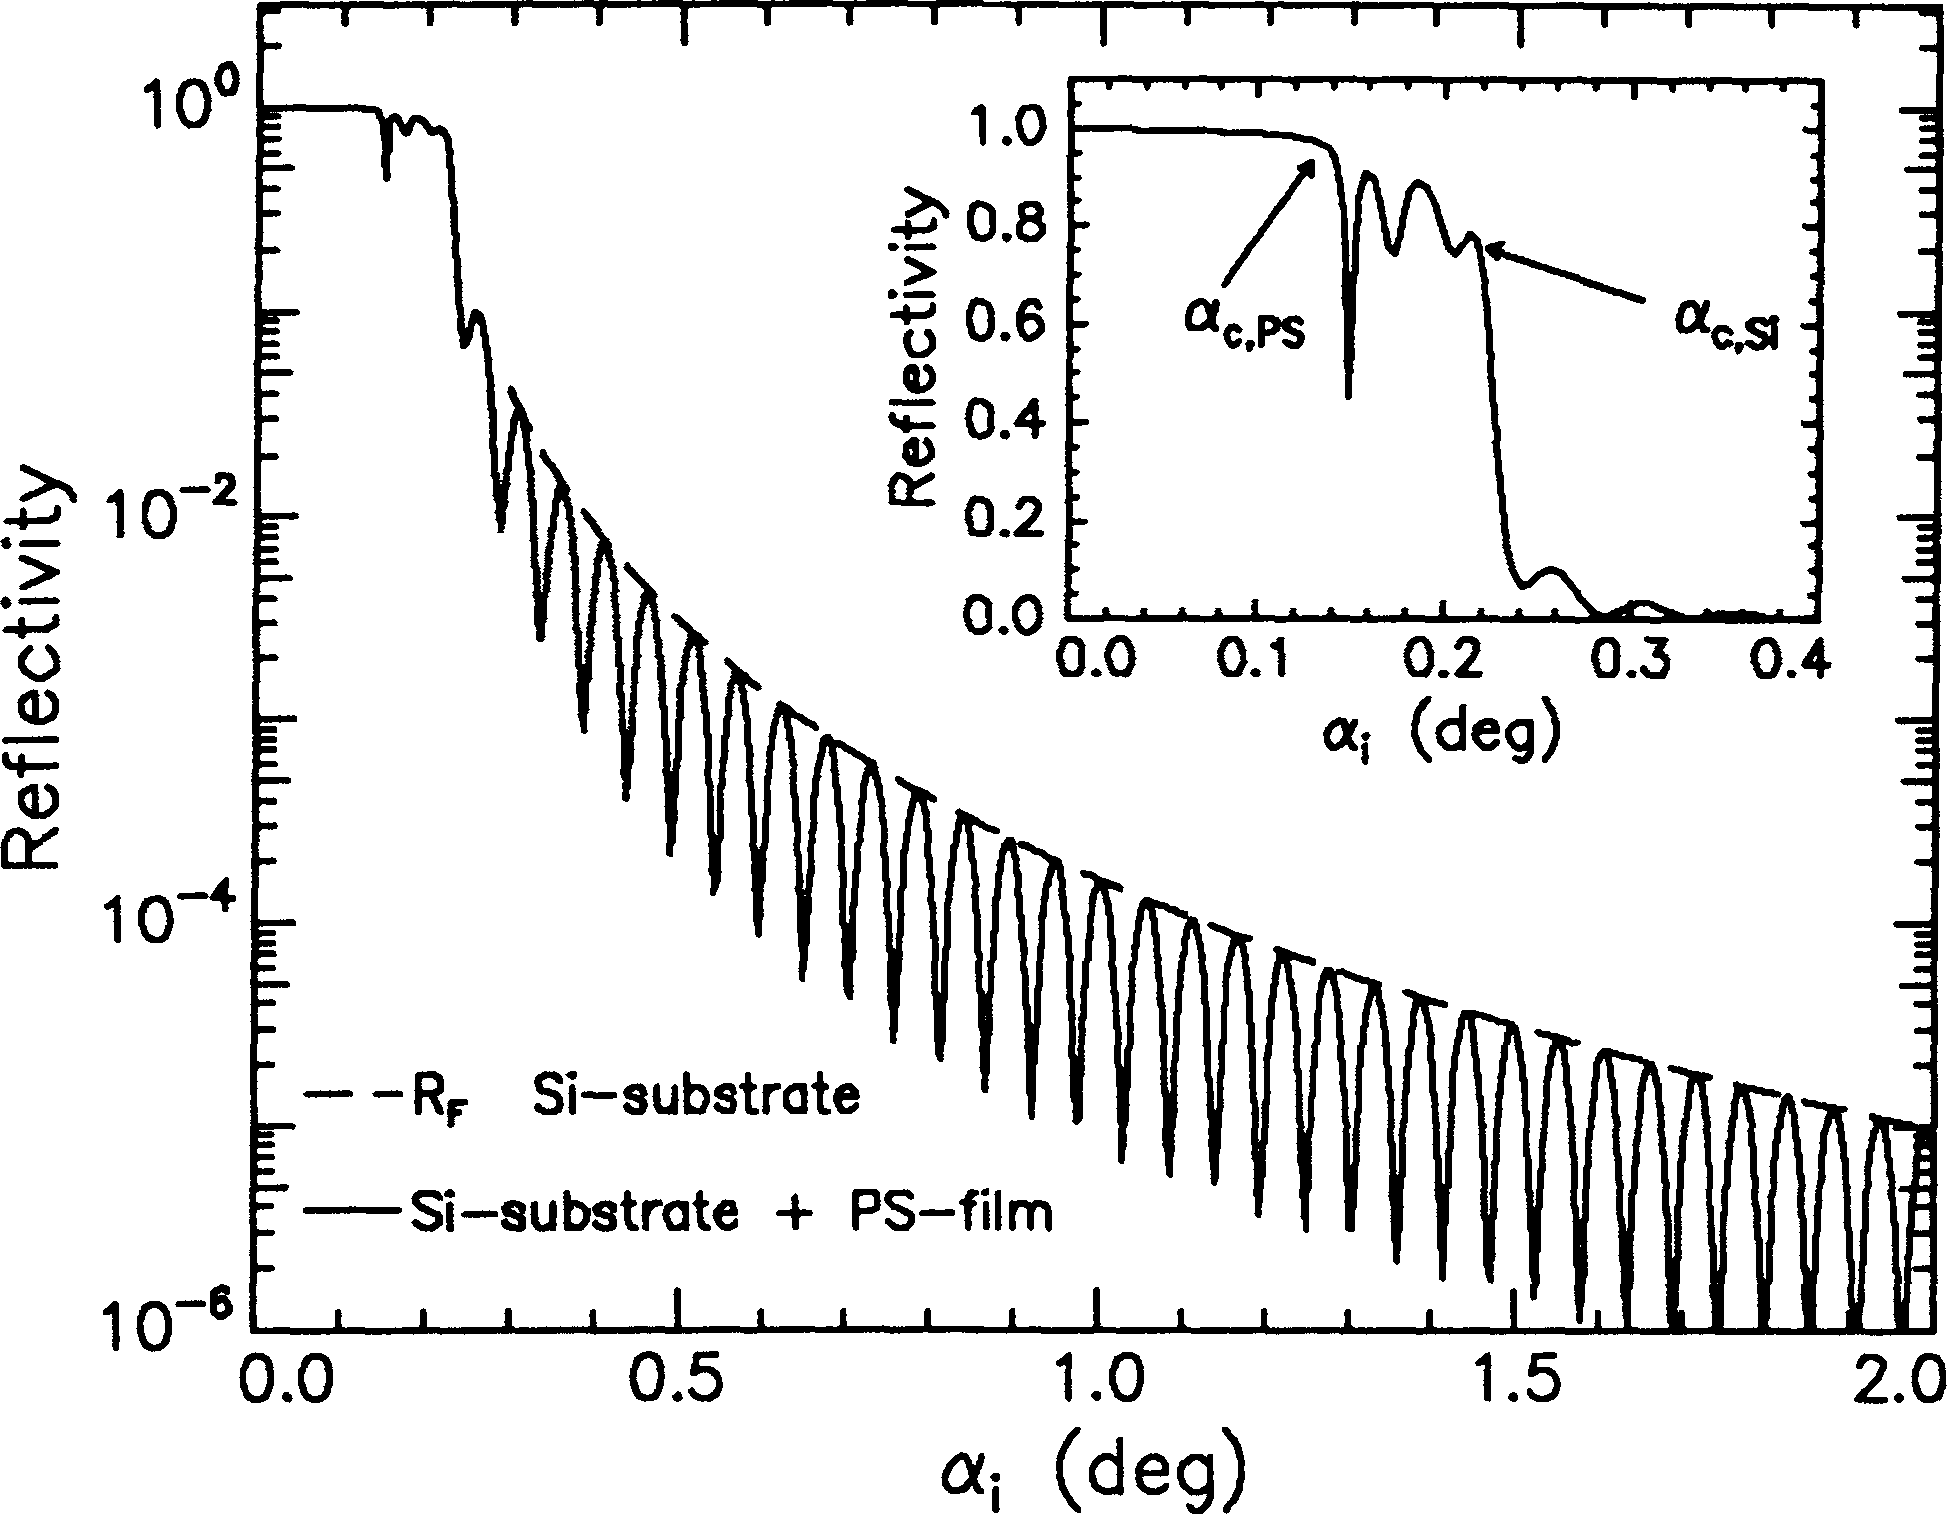
\includegraphics[width=\textwidth]{content/img/Tolan_2.7.png}
        \caption{
            Reflektivität von Röntgenstrahlung \cite{tolan}.
            Aufgrund von Interferenzen entstehen Kiessig-Oszillationen.
        }
        \label{fig:kiessig_oszillationen}
    \end{subfigure}
\end{figure}
Aufgrund von Interferenzen zwischen den einzelnen transmittierten und reflektierten Strahlen kommt es zu sogenannten Kiessig-Oszillationen \cite{kiessig} in der beobachteten Intensität.
Dies ist in \autoref{fig:kiessig_oszillationen} gezeigt.
Aus den Abständen der einzelnen Minima oder Maxima lässt sich über die Gleichung
\begin{equation}
    d = \frac{\lambda}{2 \symup{\Delta} \alpha_i}
    \label{eqn:schichtdicke_kiessig}
\end{equation}
die Dicke der einzelnen Schichten berechnen.

Zur Abschätzung der einzelnen Schichten wird der Parratt-Algorithmus \cite{parratt} verwendet.
Dieser durchläuft rekursiv die einzelnen Schichten des Systems,
unter der Annahme,
dass die unterste Schicht unendlich dick ist.
Die Rekursionsgleichung ist durch
\begin{equation}
    X_{j} = \exp{(-2\symup{i} k_{z, j} z_{j})} \cdot
    \frac{r_{j, j+1} + X_{j+1} \exp{(2\symup{i} k_{z, j+1} z_{j})}}
    {1 + r_{j, j+1} \cdot X_{j+1} \exp{(2\symup{i} k_{z, j+1} z_{j})}}
\end{equation}
gegeben,
wobei
\begin{equation}
    r_{j, j+1} = \frac{k_{z, j} - k_{z, j+1}}{k_{z, j} + k_{z, j+1}}
\end{equation}
der Fresnel'sche Reflexionskoeffizient,
und
\begin{equation}
    k_{z, j} = k \cdot \sqrt{n^2_j - \cos^2{\alpha_i}}
\end{equation}
die z-Komponente des Wellenvektors der jeweiligen Schicht $j$ ist.

Bisher wurde die Oberfläche des Mediums als glatt angenommen.
Im Normalfall ist dies allerdings meist nicht realisiert und es muss die Rauigkeit der Oberfläche beachtet werden.
Diese wird durch
\begin{equation}
    \sigma^2_j = \int{(z-z_j) P_j(z) \symup{d}z}
\end{equation}
beschrieben,
wobei $P_j(z)$ die Wahrscheinlichkeit bezeichnet,
dass die Grenzfläche mit dem Index $j$ in einem Intervall $(z_j + z, z_j + z + \symup{d}z)$ liegt.
Unter Berücksichtigung der Rauigkeit der Oberflächen ergeben sich Korrekturen in den Reflexions- und Transmissionskoeffizienten.
Es gilt
\begin{gather}
    \bar{r}_{j, j+1} = r_{j, j+1} \exp{(-2 k_{z, j} k_{z, j+1} \sigma^2_{j})} \\
    \bar{t}_{j, j+1} = t_{j, j+1} \exp{\biggl((k_{z, j} - k_{z, j+1}) \frac{\sigma^2_{j}}{2}\biggr)} \ .
\end{gather}
